
\documentclass{article}

% Required packages
\usepackage{amssymb}
\usepackage{amsmath}
\usepackage{graphicx}
\usepackage{geometry}
\usepackage{tikz}
\usepackage{array}
\usepackage{booktabs}
\usepackage{enumitem}
\usepackage{listings}
\usepackage{xcolor}
\usepackage{fancyhdr}
\usepackage{float}
\usepackage{subcaption}

% Set page geometry
\geometry{a4paper, margin=1in}

% Configure listings for Python
\lstset{
  language=Python,
  basicstyle=\ttfamily\footnotesize,
  numbers=left,
  numberstyle=\tiny\color{gray},
  frame=single,
  breaklines=true,
  breakatwhitespace=true,
  captionpos=b,
  tabsize=4,
  showspaces=false,
  showstringspaces=false,
  showtabs=false,
  commentstyle=\color{gray}\textit,
  keywordstyle=\color{blue}\bfseries,
  stringstyle=\color{red}
}

\begin{document}

\pagestyle{fancy}
\chead{DSC 255: Machine Learning Fundamentals (Spring 2025)}
\lhead{Homework 6}
\rhead{Randall Rogers}

\subsection*{Solution 1}
\noindent\rule{\textwidth}{0.4pt}\\

\subsubsection*{Step 1}
\parbox{\textwidth}{
The prediction rule is given by $\left(2 x_{1}-x_{2}-6\right)$. In a linear classifier, the decision boundary is where the prediction rule equals zero:
$$2 x_{1}-x_{2}-6 = 0$$

We can rearrange this to express $x_2$ in terms of $x_1$:
$$x_{2} = 2 x_{1} - 6$$

This is the equation of our decision boundary in $\mathbb{R}^{2}$.
}

\subsubsection*{Step 2}
\parbox{\textwidth}{
To find where the decision boundary intersects the axes:

\textbf{x-axis intersection} (where $x_2 = 0$):
$$0 = 2x_1 - 6$$
$$2x_1 = 6$$
$$x_1 = 3$$

So the boundary intersects the x-axis at the point $(3, 0)$.

\textbf{y-axis intersection} (where $x_1 = 0$):
$$x_2 = 2(0) - 6$$
$$x_2 = -6$$

So the boundary intersects the y-axis at the point $(0, -6)$.
}

\subsubsection*{Step 3}
\parbox{\textwidth}{
To determine which side of the boundary is classified as positive and which as negative, we need to examine the sign of the prediction rule $f(x) = 2x_1 - x_2 - 6$.

For a point $(x_1, x_2)$:
\begin{itemize}
    \item If $2x_1 - x_2 - 6 > 0$, the point is classified as positive.
    \item If $2x_1 - x_2 - 6 < 0$, the point is classified as negative.
\end{itemize}

Let's test a point clearly on one side of the line, such as the origin $(0,0)$:
$$f(0,0) = 2(0) - 0 - 6 = -6 < 0$$

So the origin is classified as negative. This means:
\begin{itemize}
    \item The region below the line $x_2 = 2x_1 - 6$ is classified as positive.
    \item The region above the line $x_2 = 2x_1 - 6$ is classified as negative.
\end{itemize}
}

\subsubsection*{Step 4}
\parbox{\textwidth}{
Let's visualize the decision boundary:
}

\begin{center}
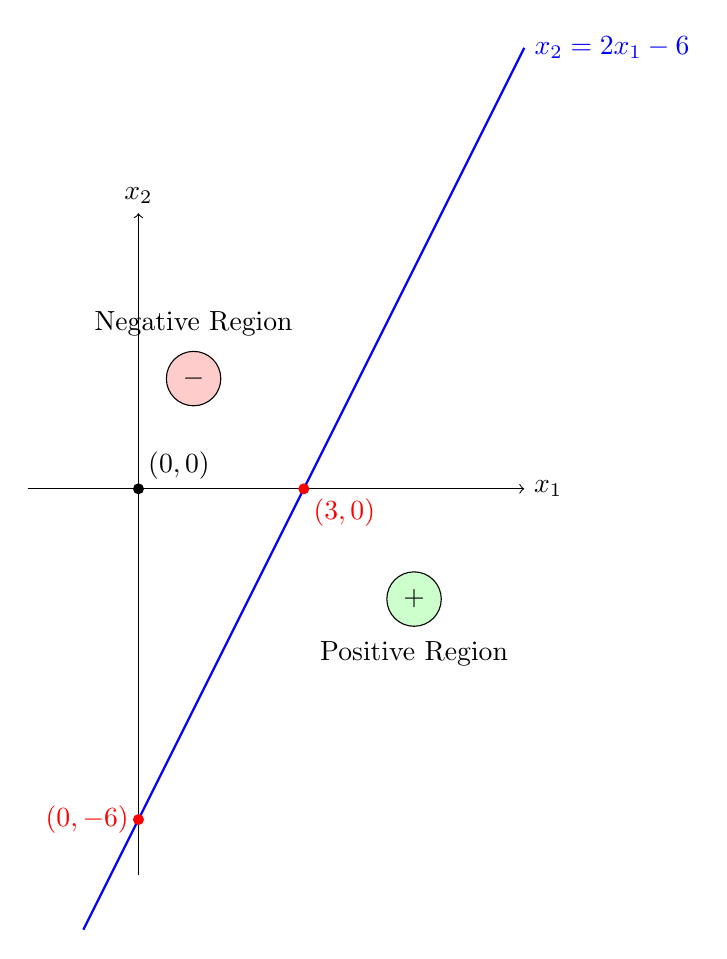
\begin{tikzpicture}[scale=0.7]
    % Draw axes
    \draw[->] (-2,0) -- (7,0) node[right] {$x_1$};
    \draw[->] (0,-7) -- (0,5) node[above] {$x_2$};
    
    % Draw decision boundary
    \draw[blue, thick] (-1,-8) -- (7,8) node[right] {$x_2 = 2x_1 - 6$};
    
    % Mark intersections
    \fill[red] (3,0) circle (0.1) node[below right] {$(3,0)$};
    \fill[red] (0,-6) circle (0.1) node[left] {$(0,-6)$};
    
    % Label regions
    \node at (5,-3) {Positive Region};
    \node at (1,3) {Negative Region};
    
    % Add + and - symbols to make it clearer
    \node[circle, draw, fill=green!20] at (5,-2) {$+$};
    \node[circle, draw, fill=red!20] at (1,2) {$-$};
    
    % Origin
    \fill[black] (0,0) circle (0.1) node[above right] {$(0,0)$};
\end{tikzpicture}
\end{center}

\subsubsection*{\normalfont}{$\therefore$ The decision boundary is the line $x_2 = 2x_1 - 6$, which intersects the x-axis at $(3,0)$ and the y-axis at $(0,-6)$. The region below this line is classified as positive, and the region above it is classified as negative.}

\noindent\rule{\textwidth}{0.4pt}\\

\newpage

\subsection*{Solution 2 (a)}
\noindent\rule{\textwidth}{0.4pt}\\

\subsubsection*{Step 1}
\parbox{\textwidth}{
The question states that the Perceptron algorithm converges after making $k$ updates. We need to determine if this means the data set is definitely linearly separable.
}

\subsubsection*{Step 2}
\parbox{\textwidth}{
Recall the Perceptron Convergence Theorem: If a dataset is linearly separable, the Perceptron algorithm is guaranteed to converge in a finite number of updates.

However, the converse is not necessarily true. If the Perceptron algorithm converges, it only means that it found a hyperplane that correctly classifies the training data it has seen, but this doesn't guarantee that the entire dataset is linearly separable.

In this case, since we're told that the algorithm converges after cycling through all points repeatedly until convergence, this implies that the algorithm has seen all data points and found a hyperplane that correctly classifies all of them.
}

\subsubsection*{\normalfont}{$\therefore$ The statement "The data set is linearly separable" is \textbf{definitely true}. The Perceptron algorithm converges if and only if the data is linearly separable. Since we're told it converges after cycling through all points repeatedly, this means a separating hyperplane exists for the entire dataset.}

\noindent\rule{\textwidth}{0.4pt}\\

\newpage

\subsection*{Solution 2 (b)}
\noindent\rule{\textwidth}{0.4pt}\\

\subsubsection*{Step 1}
\parbox{\textwidth}{
The question asks whether the Perceptron algorithm would again converge if run with a different random permutation of the same dataset.
}

\subsubsection*{Step 2}
\parbox{\textwidth}{
From part (a), we established that the dataset is linearly separable. The Perceptron Convergence Theorem guarantees that for any linearly separable dataset, the Perceptron algorithm will converge in a finite number of updates, regardless of the order in which the data points are presented.

The order of presentation (permutation) may affect the specific hyperplane found and the number of updates required, but it does not affect whether the algorithm converges.
}

\subsubsection*{\normalfont}{$\therefore$ The statement "If the process were repeated with a different random permutation, it would again converge" is \textbf{definitely true}. Since the dataset is linearly separable, the Perceptron algorithm will converge regardless of the order in which the data points are presented.}

\noindent\rule{\textwidth}{0.4pt}\\

\newpage

\subsection*{Solution 2 (c)}
\noindent\rule{\textwidth}{0.4pt}\\

\subsubsection*{Step 1}
\parbox{\textwidth}{
The question asks whether the Perceptron algorithm would converge after exactly $k$ updates if run with a different random permutation of the same dataset.
}

\subsubsection*{Step 2}
\parbox{\textwidth}{
The number of updates required for the Perceptron algorithm to converge depends on several factors:
\begin{itemize}
    \item The specific data points and their labels
    \item The order in which the data points are presented
    \item The initial weight vector
    \item The margin of separation in the data
\end{itemize}

Different permutations of the data can lead to different update sequences and potentially different numbers of updates before convergence. While the algorithm will still converge (as established in part (b)), there is no guarantee that it will make exactly $k$ updates with a different permutation.
}

\subsubsection*{\normalfont}{$\therefore$ The statement "If the process were repeated with a different random permutation, it would again converge after making $k$ updates" is \textbf{possibly false}. The number of updates required for convergence can vary depending on the specific permutation of the data.}

\noindent\rule{\textwidth}{0.4pt}\\

\newpage

\subsection*{Solution 2 (d)}
\noindent\rule{\textwidth}{0.4pt}\\

\subsubsection*{Step 1}
\parbox{\textwidth}{
The question asks whether $k$ (the number of updates until convergence) is at most $n$ (the number of data points).
}

\subsubsection*{Step 2}
\parbox{\textwidth}{
In the Perceptron algorithm, an update occurs only when a data point is misclassified. In the worst case, every data point could be misclassified in each complete cycle through the dataset.

The algorithm cycles through all $n$ points repeatedly until convergence. If it takes multiple cycles to converge, then the total number of updates $k$ could be greater than $n$.

For example, if it takes 3 complete cycles through the dataset to converge, and several points are misclassified in each cycle, then $k$ could be much larger than $n$.

The Perceptron Convergence Theorem provides an upper bound on the number of updates, which depends on the margin of separation and the maximum norm of the data points, but this bound is not simply $n$.
}

\subsubsection*{\normalfont}{$\therefore$ The statement "$k$ is at most $n$" is \textbf{possibly false}. The number of updates $k$ can exceed the number of data points $n$ if multiple passes through the dataset are required for convergence.}

\noindent\rule{\textwidth}{0.4pt}\\

\newpage

\subsection*{Solution 3}
\noindent\rule{\textwidth}{0.4pt}\\

\subsubsection*{Step 1}
\parbox{\textwidth}{
Let's recall the Perceptron update rule. When a point $(x_i, y_i)$ is misclassified:

\begin{align}
w &\leftarrow w + y_i x_i\\
b &\leftarrow b + y_i
\end{align}

where $w$ is the weight vector, $b$ is the bias term, $x_i$ is the feature vector, and $y_i$ is the label ($+1$ or $-1$).
}

\subsubsection*{Step 2}
\parbox{\textwidth}{
We're told that the Perceptron algorithm performs $p+q$ updates in total:
\begin{itemize}
    \item $p$ updates on data points with label $y_i = -1$
    \item $q$ updates on data points with label $y_i = +1$
\end{itemize}

Let's assume the bias term $b$ is initialized to 0, which is a standard initialization for the Perceptron algorithm.
}

\subsubsection*{Step 3}
\parbox{\textwidth}{
For each update on a point with label $y_i = -1$, the bias is updated as:
\begin{align}
b &\leftarrow b + y_i\\
&\leftarrow b + (-1)\\
&\leftarrow b - 1
\end{align}

So after $p$ such updates, the contribution to $b$ is $-p$.

For each update on a point with label $y_i = +1$, the bias is updated as:
\begin{align}
b &\leftarrow b + y_i\\
&\leftarrow b + (+1)\\
&\leftarrow b + 1
\end{align}

So after $q$ such updates, the contribution to $b$ is $+q$.
}

\subsubsection*{Step 4}
\parbox{\textwidth}{
Combining the effects of all updates, and starting from $b = 0$:

\begin{align}
b_{\text{final}} &= 0 + (-p) + q\\
&= q - p
\end{align}
}

\subsubsection*{\normalfont}{$\therefore$ The final value of the parameter $b$ is $q - p$.}

\noindent\rule{\textwidth}{0.4pt}\\

\newpage

\subsection*{Solution 4 (a)}
\noindent\rule{\textwidth}{0.4pt}\\

\subsubsection*{Step 1}
\parbox{\textwidth}{
Given information:
\begin{itemize}
    \item SVM classifier in $\mathbb{R}^{2}$
    \item Weight vector $w = (3, 4)$
    \item Bias term $b = -12$
\end{itemize}

The decision boundary of an SVM is defined by the equation $w \cdot x + b = 0$, where $x$ is a point in the feature space.
}

\subsubsection*{Step 2}
\parbox{\textwidth}{
Substituting the given values:
\begin{align}
w \cdot x + b &= 0\\
(3, 4) \cdot (x_1, x_2) + (-12) &= 0\\
3x_1 + 4x_2 - 12 &= 0\\
3x_1 + 4x_2 &= 12
\end{align}

We can rearrange to express $x_2$ in terms of $x_1$:
\begin{align}
4x_2 &= 12 - 3x_1\\
x_2 &= 3 - \frac{3}{4}x_1
\end{align}
}

\subsubsection*{Step 3}
\parbox{\textwidth}{
To find where the decision boundary intersects the axes:

\textbf{x-axis intersection} (where $x_2 = 0$):
\begin{align}
0 &= 3 - \frac{3}{4}x_1\\
\frac{3}{4}x_1 &= 3\\
x_1 &= 4
\end{align}

So the boundary intersects the x-axis at the point $(4, 0)$.

\textbf{y-axis intersection} (where $x_1 = 0$):
\begin{align}
x_2 &= 3 - \frac{3}{4} \cdot 0\\
x_2 &= 3
\end{align}

So the boundary intersects the y-axis at the point $(0, 3)$.
}

\begin{center}
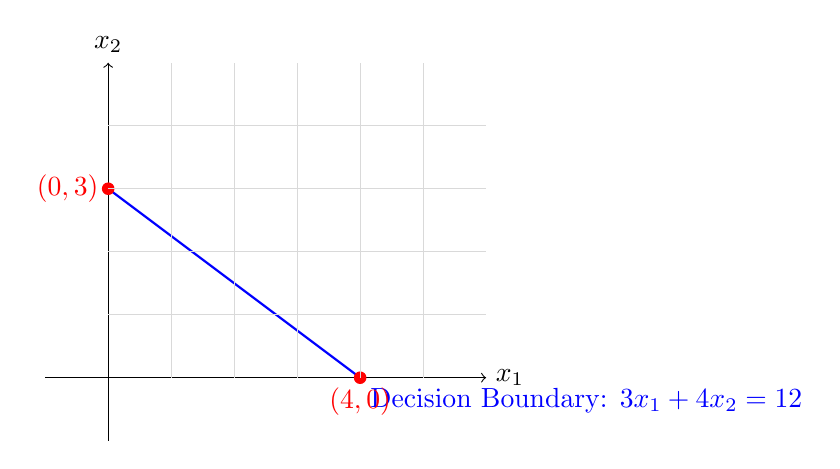
\begin{tikzpicture}[scale=0.8]
    % Draw axes
    \draw[->] (-1,0) -- (6,0) node[right] {$x_1$};
    \draw[->] (0,-1) -- (0,5) node[above] {$x_2$};
    
    % Draw decision boundary
    \draw[blue, thick] (0,3) -- (4,0) node[below right] {Decision Boundary: $3x_1 + 4x_2 = 12$};
    
    % Mark intersections
    \fill[red] (4,0) circle (0.1) node[below] {$(4,0)$};
    \fill[red] (0,3) circle (0.1) node[left] {$(0,3)$};
    
    % Add grid lines
    \draw[gray!30] (0,1) -- (6,1);
    \draw[gray!30] (0,2) -- (6,2);
    \draw[gray!30] (0,3) -- (6,3);
    \draw[gray!30] (0,4) -- (6,4);
    \draw[gray!30] (1,0) -- (1,5);
    \draw[gray!30] (2,0) -- (2,5);
    \draw[gray!30] (3,0) -- (3,5);
    \draw[gray!30] (4,0) -- (4,5);
    \draw[gray!30] (5,0) -- (5,5);
\end{tikzpicture}
\end{center}

\subsubsection*{\normalfont}{$\therefore$ The decision boundary is the line $3x_1 + 4x_2 = 12$ or equivalently $x_2 = 3 - \frac{3}{4}x_1$. It intersects the x-axis at $(4, 0)$ and the y-axis at $(0, 3)$.}

\noindent\rule{\textwidth}{0.4pt}\\

\newpage

\subsection*{Solution 4 (b)}
\noindent\rule{\textwidth}{0.4pt}\\

\subsubsection*{Step 1}
\parbox{\textwidth}{
For an SVM, the left-hand and right-hand boundaries (also called the margin boundaries) are parallel to the decision boundary and are at a distance of $\frac{1}{||w||}$ from it.

The distance from a point $(x_1, x_2)$ to the decision boundary $w \cdot x + b = 0$ is given by:
\begin{align}
d = \frac{|w \cdot x + b|}{||w||}
\end{align}

The margin boundaries are defined by the equations:
\begin{align}
w \cdot x + b &= 1 \quad \text{(positive margin boundary)}\\
w \cdot x + b &= -1 \quad \text{(negative margin boundary)}
\end{align}
}

\subsubsection*{Step 2}
\parbox{\textwidth}{
For our SVM with $w = (3, 4)$ and $b = -12$:

\textbf{Positive margin boundary:}
\begin{align}
w \cdot x + b &= 1\\
3x_1 + 4x_2 - 12 &= 1\\
3x_1 + 4x_2 &= 13\\
x_2 &= \frac{13 - 3x_1}{4} = 3.25 - \frac{3}{4}x_1
\end{align}

\textbf{Negative margin boundary:}
\begin{align}
w \cdot x + b &= -1\\
3x_1 + 4x_2 - 12 &= -1\\
3x_1 + 4x_2 &= 11\\
x_2 &= \frac{11 - 3x_1}{4} = 2.75 - \frac{3}{4}x_1
\end{align}
}

\subsubsection*{Step 3}
\parbox{\textwidth}{
Let's find where these margin boundaries intersect the axes:

\textbf{Positive margin boundary:}

x-axis intersection ($x_2 = 0$):
\begin{align}
0 &= 3.25 - \frac{3}{4}x_1\\
\frac{3}{4}x_1 &= 3.25\\
x_1 &= \frac{13}{3} \approx 4.33
\end{align}

y-axis intersection ($x_1 = 0$):
\begin{align}
x_2 &= 3.25 - \frac{3}{4} \cdot 0 = 3.25
\end{align}

\textbf{Negative margin boundary:}

x-axis intersection ($x_2 = 0$):
\begin{align}
0 &= 2.75 - \frac{3}{4}x_1\\
\frac{3}{4}x_1 &= 2.75\\
x_1 &= \frac{11}{3} \approx 3.67
\end{align}

y-axis intersection ($x_1 = 0$):
\begin{align}
x_2 &= 2.75 - \frac{3}{4} \cdot 0 = 2.75
\end{align}
}

\begin{center}
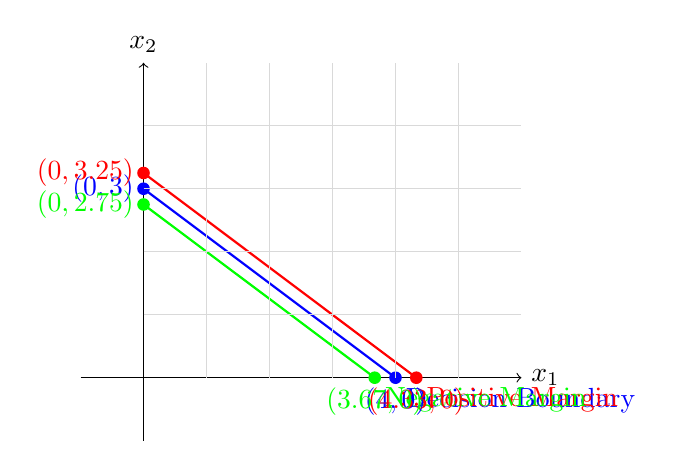
\begin{tikzpicture}[scale=0.8]
    % Draw axes
    \draw[->] (-1,0) -- (6,0) node[right] {$x_1$};
    \draw[->] (0,-1) -- (0,5) node[above] {$x_2$};
    
    % Draw decision boundary and margin boundaries
    \draw[blue, thick] (0,3) -- (4,0) node[below right] {Decision Boundary};
    \draw[red, thick] (0,3.25) -- (4.33,0) node[below right] {Positive Margin};
    \draw[green, thick] (0,2.75) -- (3.67,0) node[below right] {Negative Margin};
    
    % Mark intersections
    \fill[blue] (4,0) circle (0.1) node[below] {$(4,0)$};
    \fill[blue] (0,3) circle (0.1) node[left] {$(0,3)$};
    
    \fill[red] (4.33,0) circle (0.1) node[below] {$(4.33,0)$};
    \fill[red] (0,3.25) circle (0.1) node[left] {$(0,3.25)$};
    
    \fill[green] (3.67,0) circle (0.1) node[below] {$(3.67,0)$};
    \fill[green] (0,2.75) circle (0.1) node[left] {$(0,2.75)$};
    
    % Add grid lines
    \draw[gray!30] (0,1) -- (6,1);
    \draw[gray!30] (0,2) -- (6,2);
    \draw[gray!30] (0,3) -- (6,3);
    \draw[gray!30] (0,4) -- (6,4);
    \draw[gray!30] (1,0) -- (1,5);
    \draw[gray!30] (2,0) -- (2,5);
    \draw[gray!30] (3,0) -- (3,5);
    \draw[gray!30] (4,0) -- (4,5);
    \draw[gray!30] (5,0) -- (5,5);
\end{tikzpicture}
\end{center}

\subsubsection*{\normalfont}{$\therefore$ The positive margin boundary is the line $3x_1 + 4x_2 = 13$ or $x_2 = 3.25 - \frac{3}{4}x_1$, intersecting the x-axis at $(4.33, 0)$ and the y-axis at $(0, 3.25)$. The negative margin boundary is the line $3x_1 + 4x_2 = 11$ or $x_2 = 2.75 - \frac{3}{4}x_1$, intersecting the x-axis at $(3.67, 0)$ and the y-axis at $(0, 2.75)$.}

\noindent\rule{\textwidth}{0.4pt}\\

\newpage

\subsection*{Solution 4 (c)}
\noindent\rule{\textwidth}{0.4pt}\\

\subsubsection*{Step 1}
\parbox{\textwidth}{
The margin of an SVM classifier is defined as the perpendicular distance between the two margin boundaries, which is equal to $\frac{2}{||w||}$.

We need to calculate $||w||$, the Euclidean norm of the weight vector:
\begin{align}
||w|| &= \sqrt{w_1^2 + w_2^2}\\
&= \sqrt{3^2 + 4^2}\\
&= \sqrt{9 + 16}\\
&= \sqrt{25}\\
&= 5
\end{align}
}

\subsubsection*{Step 2}
\parbox{\textwidth}{
Now we can calculate the margin:
\begin{align}
\text{margin} &= \frac{2}{||w||}\\
&= \frac{2}{5}\\
&= 0.4
\end{align}
}

\subsubsection*{\normalfont}{$\therefore$ The margin of this SVM classifier is $\frac{2}{5} = 0.4$ units.}

\noindent\rule{\textwidth}{0.4pt}\\

\newpage

\subsection*{Solution 4 (d)}
\noindent\rule{\textwidth}{0.4pt}\\

\subsubsection*{Step 1}
\parbox{\textwidth}{
To classify a point $(x_1, x_2)$ using an SVM, we compute the sign of $w \cdot x + b$:
\begin{itemize}
    \item If $w \cdot x + b > 0$, the point is classified as positive.
    \item If $w \cdot x + b < 0$, the point is classified as negative.
    \item If $w \cdot x + b = 0$, the point lies exactly on the decision boundary.
\end{itemize}
}

\subsubsection*{Step 2}
\parbox{\textwidth}{
For the point $(2, 2)$ with $w = (3, 4)$ and $b = -12$:
\begin{align}
w \cdot x + b &= 3 \cdot 2 + 4 \cdot 2 + (-12)\\
&= 6 + 8 - 12\\
&= 14 - 12\\
&= 2 > 0
\end{align}
}

\subsubsection*{Step 3}
\parbox{\textwidth}{
We can also verify this geometrically. The decision boundary is the line $3x_1 + 4x_2 = 12$. For the point $(2, 2)$:
\begin{align}
3 \cdot 2 + 4 \cdot 2 = 6 + 8 = 14 > 12
\end{align}

This confirms that the point lies on the positive side of the decision boundary.
}

\begin{center}
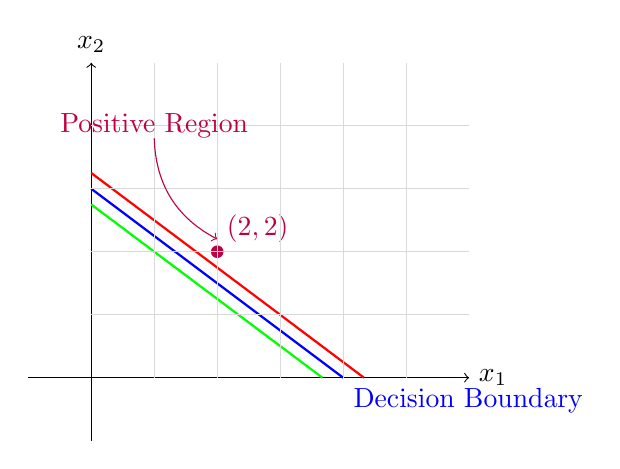
\begin{tikzpicture}[scale=0.8]
    % Draw axes
    \draw[->] (-1,0) -- (6,0) node[right] {$x_1$};
    \draw[->] (0,-1) -- (0,5) node[above] {$x_2$};
    
    % Draw decision boundary and margin boundaries
    \draw[blue, thick] (0,3) -- (4,0) node[below right] {Decision Boundary};
    \draw[red, thick] (0,3.25) -- (4.33,0);
    \draw[green, thick] (0,2.75) -- (3.67,0);
    
    % Mark the point (2,2)
    \fill[purple] (2,2) circle (0.1) node[above right] {$(2,2)$};
    
    % Add grid lines
    \draw[gray!30] (0,1) -- (6,1);
    \draw[gray!30] (0,2) -- (6,2);
    \draw[gray!30] (0,3) -- (6,3);
    \draw[gray!30] (0,4) -- (6,4);
    \draw[gray!30] (1,0) -- (1,5);
    \draw[gray!30] (2,0) -- (2,5);
    \draw[gray!30] (3,0) -- (3,5);
    \draw[gray!30] (4,0) -- (4,5);
    \draw[gray!30] (5,0) -- (5,5);
    
    % Indicate positive region
    \node[text=purple] at (1,4) {Positive Region};
    \draw[purple, ->] (1,3.8) to[bend right] (2,2.2);
\end{tikzpicture}
\end{center}

\subsubsection*{\normalfont}{$\therefore$ The point $(2, 2)$ would be classified as \textbf{positive} because $w \cdot x + b = 2 > 0$.}

\noindent\rule{\textwidth}{0.4pt}\\

\newpage

\subsection*{Solution 5 (a)}
\noindent\rule{\textwidth}{0.4pt}\\

\subsubsection*{Step 1}
\parbox{\textwidth}{
In a soft-margin SVM, the support vectors are the data points that:
\begin{itemize}
    \item Lie exactly on the margin boundaries (slack variable $\xi_i = 0$)
    \item Lie between the margin boundary and the decision boundary (slack variable $0 < \xi_i < 1$)
    \item Lie on the wrong side of the margin boundary (slack variable $\xi_i \geq 1$)
\end{itemize}

The slack variable $\xi_i$ represents the degree of misclassification for each point. It measures how far a point is from its correct margin boundary.
}

\subsubsection*{Step 2}
\parbox{\textwidth}{
Let's identify the support vectors in the given figure:

\begin{center}
  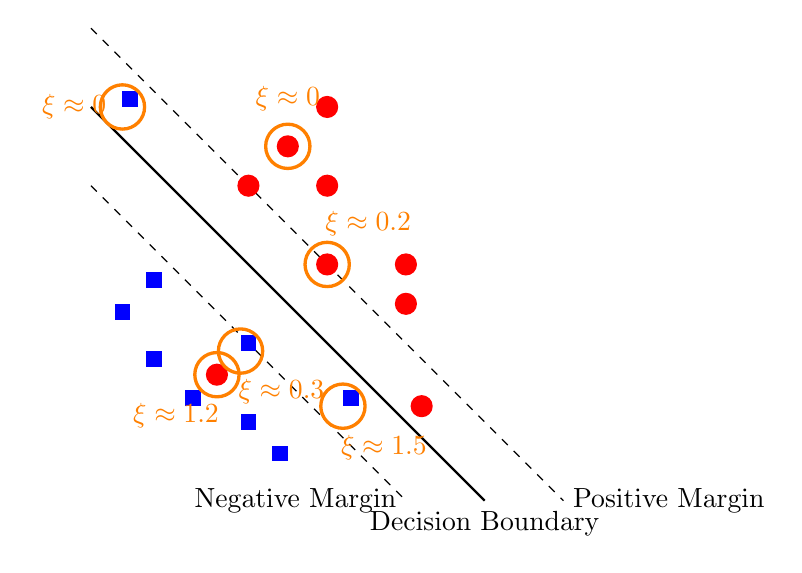
\begin{tikzpicture}
  % Solid decision boundary (approx. average of lines)
  \draw[thick] (0,5) -- (5,0) node[below] {Decision Boundary};
  \draw[dashed] (0,6) -- (6,0) node[right] {Positive Margin};
  \draw[dashed] (0,4) -- (4,0) node[left] {Negative Margin};

  % Blue squares (negative class)
  \foreach \x/\y in {0.7/2.7,0.7/1.7, 0.3/2.3,1.2/1.2,1.9/0.9,2.3/0.5 ,1.9/1.9, 3.2/1.2, 0.4/5.0} {
    \fill[blue] (\x,\y) rectangle ++(0.2,0.2);}

  % Red circles (positive class)
  \foreach \x/\y in {1.6/1.6, 4.2/1.2, 2/4, 3/3,3/4,3/5,2.5/4.5, 4/3,4/2.5} {
    \fill[red] (\x,\y) circle (4pt);}
    
  % Highlight support vectors and add slack variable values
  % Support vectors on or near margin boundaries (ξ = 0)
  \draw[orange, very thick, circle] (0.4,5.0) circle (8pt) node[left] {$\xi \approx 0$};
  \draw[orange, very thick, circle] (2.5,4.5) circle (8pt) node[above] {$\xi \approx 0$};
  
  % Support vectors between margin and decision boundary (0 < ξ < 1)
  \draw[orange, very thick, circle] (1.9,1.9) circle (8pt) node[below right] {$\xi \approx 0.3$};
  \draw[orange, very thick, circle] (3,3) circle (8pt) node[above right] {$\xi \approx 0.2$};
  
  % Support vectors on wrong side of margin (ξ ≥ 1)
  \draw[orange, very thick, circle] (1.6,1.6) circle (8pt) node[below left] {$\xi \approx 1.2$};
  \draw[orange, very thick, circle] (3.2,1.2) circle (8pt) node[below right] {$\xi \approx 1.5$};
  
  \end{tikzpicture}
\end{center}
}

\subsubsection*{Step 3}
\parbox{\textwidth}{
Let's explain the identified support vectors:

\begin{enumerate}
    \item \textbf{Support vectors with $\xi \approx 0$:}
    \begin{itemize}
        \item The blue square at approximately $(0.4, 5.0)$ lies very close to the negative margin boundary.
        \item The red circle at approximately $(2.5, 4.5)$ lies very close to the positive margin boundary.
        \item These points have slack variables close to zero because they are almost exactly on their respective margin boundaries.
    \end{itemize}
    
    \item \textbf{Support vectors with $0 < \xi < 1$:}
    \begin{itemize}
        \item The blue square at approximately $(1.9, 1.9)$ is between the negative margin and the decision boundary.
        \item The red circle at approximately $(3, 3)$ is between the positive margin and the decision boundary.
        \item These points have slack variables between 0 and 1 because they are inside the margin but on the correct side of the decision boundary.
    \end{itemize}
    
    \item \textbf{Support vectors with $\xi \geq 1$:}
    \begin{itemize}
        \item The red circle at approximately $(1.6, 1.6)$ is on the wrong side of the decision boundary.
        \item The blue square at approximately $(3.2, 1.2)$ is also on the wrong side of the decision boundary.
        \item These points have slack variables greater than or equal to 1 because they are misclassified by the decision boundary.
    \end{itemize}
\end{enumerate}
}

\subsubsection*{\normalfont}{$\therefore$ The support vectors are the points circled in orange in the figure above, with their approximate slack variable values indicated. Support vectors include points exactly on the margin boundaries ($\xi \approx 0$), points between the margin and decision boundary ($0 < \xi < 1$), and misclassified points ($\xi \geq 1$).}

\noindent\rule{\textwidth}{0.4pt}\\

\newpage

\subsection*{Solution 5 (b)}
\noindent\rule{\textwidth}{0.4pt}\\

\subsubsection*{Step 1}
\parbox{\textwidth}{
Recall the optimization problem for soft-margin SVM:

$$\min_{w, b, \xi} \frac{1}{2} ||w||^2 + C \sum_{i=1}^{n} \xi_i$$

subject to:
$$y_i(w \cdot x_i + b) \geq 1 - \xi_i, \quad \xi_i \geq 0 \quad \forall i$$

The parameter $C$ controls the trade-off between maximizing the margin (minimizing $||w||^2$) and minimizing the classification error (minimizing $\sum \xi_i$).
}

\subsubsection*{Step 2}
\parbox{\textwidth}{
When $C$ is increased:
\begin{itemize}
    \item The penalty for misclassification and margin violations becomes higher.
    \item The optimization will prioritize reducing the slack variables $\xi_i$ over maximizing the margin.
    \item This means the model will try harder to correctly classify all training points, potentially at the expense of a smaller margin.
\end{itemize}
}

\subsubsection*{Step 3}
\parbox{\textwidth}{
Let's compare the effects of different values of $C$:

\begin{center}
\begin{tabular}{|c|c|c|}
\hline
\textbf{Small $C$} & \textbf{Medium $C$} & \textbf{Large $C$} \\
\hline
Larger margin & Balanced trade-off & Smaller margin \\
More misclassifications & Some misclassifications & Fewer misclassifications \\
Underfitting risk & Good generalization & Overfitting risk \\
\hline
\end{tabular}
\end{center}

In our specific example, increasing $C$ would likely:
\begin{itemize}
    \item Make the decision boundary adjust to reduce the misclassifications (the red circle at $(1.6, 1.6)$ and the blue square at $(3.2, 1.2)$).
    \item Potentially reduce the margin between the dashed lines to better accommodate the training points.
\end{itemize}
}

\begin{center}
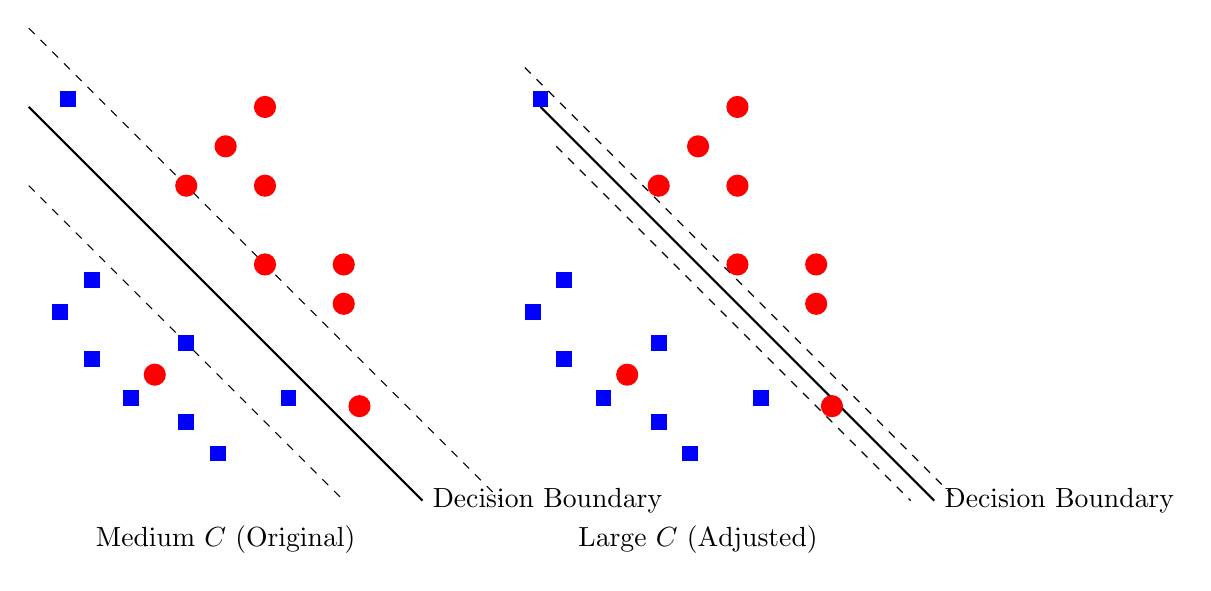
\begin{tikzpicture}
% Original SVM (medium C)
\begin{scope}[xshift=-3cm]
  \draw[thick] (0,5) -- (5,0) node[right] {Decision Boundary};
  \draw[dashed] (0,6) -- (6,0);
  \draw[dashed] (0,4) -- (4,0);
  
  % Blue squares
  \foreach \x/\y in {0.7/2.7,0.7/1.7, 0.3/2.3,1.2/1.2,1.9/0.9,2.3/0.5 ,1.9/1.9, 3.2/1.2, 0.4/5.0} {
    \fill[blue] (\x,\y) rectangle ++(0.2,0.2);}

  % Red circles
  \foreach \x/\y in {1.6/1.6, 4.2/1.2, 2/4, 3/3,3/4,3/5,2.5/4.5, 4/3,4/2.5} {
    \fill[red] (\x,\y) circle (4pt);}
    
  \node at (2.5,-0.5) {Medium $C$ (Original)};
\end{scope}

% Large C SVM
\begin{scope}[xshift=3cm]
  % Adjusted decision boundary for larger C
  \draw[thick] (0.5,5) -- (5.5,0) node[right] {Decision Boundary};
  \draw[dashed] (0.3,5.5) -- (5.8,0);
  \draw[dashed] (0.7,4.5) -- (5.2,0);
  
  % Blue squares
  \foreach \x/\y in {0.7/2.7,0.7/1.7, 0.3/2.3,1.2/1.2,1.9/0.9,2.3/0.5 ,1.9/1.9, 3.2/1.2, 0.4/5.0} {
    \fill[blue] (\x,\y) rectangle ++(0.2,0.2);}

  % Red circles
  \foreach \x/\y in {1.6/1.6, 4.2/1.2, 2/4, 3/3,3/4,3/5,2.5/4.5, 4/3,4/2.5} {
    \fill[red] (\x,\y) circle (4pt);}
    
  \node at (2.5,-0.5) {Large $C$ (Adjusted)};
\end{scope}
\end{tikzpicture}
\end{center}

\subsubsection*{\normalfont}{$\therefore$ If the factor $C$ in the soft-margin SVM optimization problem were increased, we would expect the margin to \textbf{decrease}. This is because a larger $C$ places more emphasis on correctly classifying all training points, even if it means having a smaller margin.}

\noindent\rule{\textwidth}{0.4pt}\\

\newpage

\subsection*{Solution 6 (a)}
\noindent\rule{\textwidth}{0.4pt}\\

\subsubsection*{Step 1}
\parbox{\textwidth}{
Let's recall the dual form of the Perceptron algorithm:

In the dual form, we represent the weight vector $w$ as a linear combination of the training examples:
$$w = \sum_{i=1}^{n} \alpha_i y_i x_i$$

where $\alpha_i$ counts how many times example $i$ has been misclassified during training.
}

\subsubsection*{Step 2}
\parbox{\textwidth}{
In the standard Perceptron algorithm, when a point $(x_i, y_i)$ is misclassified, we update:
$$w \leftarrow w + y_i x_i$$

In the dual form, this corresponds to incrementing $\alpha_i$ by 1:
$$\alpha_i \leftarrow \alpha_i + 1$$

Initially, all $\alpha_i$ values are set to 0. Each time a point is misclassified, its corresponding $\alpha_i$ is incremented by 1.
}

\subsubsection*{Step 3}
\parbox{\textwidth}{
Since the algorithm performs $k$ updates in total, and each update increments exactly one $\alpha_i$ by 1, we know that:

\begin{itemize}
    \item Each $\alpha_i$ represents the number of times example $i$ was misclassified
    \item Each $\alpha_i$ must be a non-negative integer
    \item Some examples might never be misclassified, so their $\alpha_i$ remains 0
    \item Some examples might be misclassified multiple times, so their $\alpha_i$ could be greater than 1
\end{itemize}
}

\subsubsection*{\normalfont}{$\therefore$ The statement "Each $\alpha_i$ is either 0 or 1" is \textbf{possibly false}. While some $\alpha_i$ values may be 0 (never misclassified) or 1 (misclassified once), it's possible for an example to be misclassified multiple times during training, resulting in $\alpha_i > 1$.}

\noindent\rule{\textwidth}{0.4pt}\\

\newpage

\subsection*{Solution 6 (b)}
\noindent\rule{\textwidth}{0.4pt}\\

\subsubsection*{Step 1}
\parbox{\textwidth}{
We know that the Perceptron algorithm makes a total of $k$ updates, and each update corresponds to incrementing exactly one $\alpha_i$ by 1.
}

\subsubsection*{Step 2}
\parbox{\textwidth}{
Initially, all $\alpha_i$ values are set to 0. After $k$ updates, each incrementing one $\alpha_i$ by 1, the sum of all $\alpha_i$ values must be equal to $k$:

$$\sum_{i=1}^{n} \alpha_i = k$$

This is because each update contributes exactly 1 to the sum of $\alpha_i$ values, and there are $k$ updates in total.
}

\subsubsection*{\normalfont}{$\therefore$ The statement "$\sum_{i} \alpha_i = k$" is \textbf{necessarily true}. Since each of the $k$ updates increments exactly one $\alpha_i$ by 1, and all $\alpha_i$ values start at 0, the sum of all $\alpha_i$ values must equal $k$.}

\noindent\rule{\textwidth}{0.4pt}\\

\newpage

\subsection*{Solution 6 (c)}
\noindent\rule{\textwidth}{0.4pt}\\

\subsubsection*{Step 1}
\parbox{\textwidth}{
We need to determine the maximum number of nonzero coordinates in the vector $\alpha$.
}

\subsubsection*{Step 2}
\parbox{\textwidth}{
A coordinate $\alpha_i$ is nonzero if and only if the corresponding example $(x_i, y_i)$ has been misclassified at least once during training.

In the worst case, each of the $k$ updates could be applied to a different example, resulting in $k$ different examples having their $\alpha_i$ incremented to 1.

However, it's also possible that some examples are misclassified multiple times, which would result in fewer than $k$ nonzero coordinates in $\alpha$.
}

\subsubsection*{Step 3}
\parbox{\textwidth}{
Let's consider a simple example to illustrate:

Suppose we have 5 training examples and the algorithm makes $k = 3$ updates:
\begin{itemize}
    \item If the updates are applied to examples 1, 2, and 3, then $\alpha = (1, 1, 1, 0, 0)$ with 3 nonzero coordinates.
    \item If the updates are applied to examples 1, 1, and 2, then $\alpha = (2, 1, 0, 0, 0)$ with 2 nonzero coordinates.
\end{itemize}

In general, the number of nonzero coordinates in $\alpha$ is at most $k$ (when each update is applied to a different example) and at least 1 (when all updates are applied to the same example).
}

\subsubsection*{\normalfont}{$\therefore$ The statement "$\alpha$ has at most $k$ nonzero coordinates" is \textbf{necessarily true}. Since there are $k$ updates in total, at most $k$ different examples can be misclassified, resulting in at most $k$ nonzero $\alpha_i$ values.}

\noindent\rule{\textwidth}{0.4pt}\\

\newpage

\subsection*{Solution 6 (d)}
\noindent\rule{\textwidth}{0.4pt}\\

\subsubsection*{Step 1}
\parbox{\textwidth}{
We need to determine whether the convergence of the Perceptron algorithm implies that the training data is linearly separable.
}

\subsubsection*{Step 2}
\parbox{\textwidth}{
Recall the Perceptron Convergence Theorem: If the training data is linearly separable, then the Perceptron algorithm will converge in a finite number of updates.

The converse is also true: If the Perceptron algorithm converges, then the training data must be linearly separable. This is because:

\begin{itemize}
    \item Convergence means the algorithm has found a weight vector $w$ and bias $b$ such that all training examples are correctly classified.
    \item This means there exists a hyperplane defined by $w \cdot x + b = 0$ that separates the positive and negative examples.
    \item By definition, this makes the data linearly separable.
\end{itemize}
}

\subsubsection*{Step 3}
\parbox{\textwidth}{
It's important to note that if the data is not linearly separable, the Perceptron algorithm will never converge - it will continue to make updates indefinitely as it cycles through the data.

Since we're told that the algorithm converges after $k$ updates, this implies that the algorithm has found a separating hyperplane, which means the data must be linearly separable.
}

\subsubsection*{\normalfont}{$\therefore$ The statement "The training data must be linearly separable" is \textbf{necessarily true}. The convergence of the Perceptron algorithm implies that it has found a hyperplane that correctly classifies all training examples, which by definition means the data is linearly separable.}

\noindent\rule{\textwidth}{0.4pt}\\

\newpage
\begin{center}
  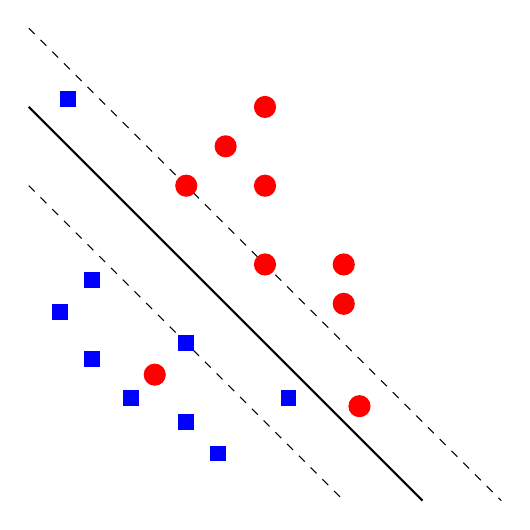
\begin{tikzpicture}
  % Solid decision boundary (approx. average of lines)
  \draw[thick] (0,5) -- (5,0);
  \draw[dashed] (0,6) -- (6,0);
  \draw[dashed] (0,4) -- (4,0);

  % Blue squares
  \foreach \x/\y in {0.7/2.7,0.7/1.7, 0.3/2.3,1.2/1.2,1.9/0.9,2.3/0.5 ,1.9/1.9, 3.2/1.2, 0.4/5.0} {
    \fill[blue] (\x,\y) rectangle ++(0.2,0.2);}

  % Red circles
  \foreach \x/\y in {1.6/1.6, 4.2/1.2, 2/4, 3/3,3/4,3/5,2.5/4.5, 4/3,4/2.5} {
    \fill[red] (\x,\y) circle (4pt);}
  \end{tikzpicture}
\end{center}

\end{document}
